\documentclass[letterpaper,12pt,fleqn]{article}
\usepackage{matharticle}
\usepackage{amsfonts}
\usepackage{mathtools}
\usepackage{tikz}

\begin{document}

\section*{Sets}

We will be using sets to identify parts of the real number line. We start with a
somewhat complicated and unfortunately incomplete and circular definition:

\begin{definition}[Set]
A set is a \emph{well-defined}, \emph{distinct}, and \emph{unordered}
collection of members called elements, where the elements are selected from
an all-inclusive set called a universe.
\end{definition}

The definition is poor because it uses ``set'' in the definition, and
incomplete because it appeals to the reader's intuition of what it means to be
a collection and a member of a collection. There are branches of set theory
that attempt to resolve these problems; however, that is way beyond our needs
here. As it is, this approach to sets is often referred to as naive set theory.

How a set differs from just a collection is explained by the three emphasized
adjectives in the definition:

\begin{description}
\item[well-defined:] Each element in the universe is unambiguously either an
element or not an element of the set. For example, let's assume that the
universe is all integers and then define the set:
\[\{1, 2, 3\}\]
This set unambiguously contains the elements 1, 2, and 3, and nothing else. If
you are asked if 2 is in the set, you can say yes. If you are asked if 5 is in
the set you can say no. If you are asked if $\pi$ is in the set you can also
say no, because $\pi$ isn't even in the universe. However, the set:
\[\{x|x\ \mbox{is a large number}\}\]
is ambiguous. If you are asked if 100 is in the set, it is not clear whether or
not 100 qualifies as ``large'' in the mind of the person that devised the set.

\item[distinct:] Elements are not replicated. For example, the sets:
\[\{1, 2, 3\}\]
\[\{1, 2, 3, 2\}\]
are the same set. In fact, the latter set is poorly formed; we never list
duplicated elements.

\item[unordered:] Elements do not exist in any particular order in the set.
For example, the sets:
\[\{1, 2, 3\}\]
\[\{1, 3, 2\}\]
are the same set.
\end{description}

\subsection*{Universe}

We can use a \emph{Venn Diagram} to help us visualize a set and its relation to
a universe:

\begin{center}
\begin{tikzpicture}
\draw (0,0) rectangle (6, 4);
\draw (3, 2) circle [radius=1.5];
\node at (0.5,0.5) {$U$};
\node [above] at (3,1) {A};
\end{tikzpicture}
\end{center}

The diagram shows a set A contained in a universe $U$. We typically use capital
letters to represent sets. Everything within the circle is an element of the
set. Everything in the box but not in the circle is not an element of the set.

Note that the choice of a universe is arbitrary (as long as it can contain the
desired set) and is usually driven by the problem at hand.

\subsection*{Elements}

The notation to show that $a$ is an element in a set $A$ is as follows:
\[a\in A\]
To say that $a$ is not an element in set $A$:
\[a\notin A\]
Note that since sets are well-defined, $a\in A\ or\ a\notin A$ must be a true
statement (something is unambiguously either in or not in the set).

For example, if we choose our universe to be the set of natural numbers
$\mathbb{N}$ and let $A=\{1, 2, 3\}$, then $2\in A$ and $4\notin A$. A statement
like $\pi\notin A$ is true, but a bit nonsensical because $\pi$ is not even in
our selected universe.

The empty set is the set with no elements, denoted as follows:
\[\emptyset=\{\}\]
For all elements $a$ in a universe, $a\notin\emptyset$.

\subsection*{Specification}

Sets can be specified in any of the following ways:

\begin{itemize}
\item Description
\item Roster
\item Setbuilder Notation
\end{itemize}

\subsubsection*{Description}

We can describe a set using just words. Some examples are:
\begin{itemize}
\item The set of natural numbers from 2 to 5
\item The set of irrational numbers
\item The set of students in Math-19 for Spring 2016 at SJSU
\end{itemize}
We typically only use this method when we want to conceptually describe a set.
When we want to be mathematically precise, we will use one of the other
methods.

\subsubsection*{Roster}

To describe a set by roster, start with a `\{', list the elements one by one,
and then finish with a `\}'. When a set is small and finite, we can usually
list all of the elements.  For example:
\[A=\{1, 2, 3\}\]
is the set consisting of the three numbers 1, 2, and 3. For larger, finite sets
with a pattern, we can establish the pattern and use an ellipsis to represent
the omitted elements. For example, the set of natural numbers from 1 to 10 can
be represented by:
\[A=\{1, 2, 3, \ldots, 10\}\]
For infinite sets, we can just leave off the terminating value. So, for the
set of natural numbers we have:
\[\mathbb{N}=\{1, 2, 3, \ldots\}\]
For the set of integers we can say:
\[\mathbb{Z}=\{\ldots, -3, -2, -1, 0, 1, 2, 3, \ldots\}\]

\subsubsection*{Setbuilder Notation}

Most of the time we will use setbuilder notation:
\[\{\mbox{\emph{universe or pattern}} | \mbox{\emph{qualifier}}\}\]
Note that there are two forms, depending on what comes before the vertical bar.
In the first form, we specify a particular universe that we are interested in,
and then we use the qualifier to pick specific elements from that universe.
For example, one way to pick out all the irrational numbers from the real
numbers would be:
\[I=\{x\in\mathbb{R}|x\notin\mathbb{Q}\}\]
Here, $x\in\mathbb{R}$ tells us that we are going to select elements $x$ from
the universe of all real numbers, and $x\notin\mathbb{Q}$ tells us that we only
what those that are not in the set of rational numbers - hence, only the
irrational numbers.

In the second form, the part before the vertical bar gives us a pattern for the
desired elements and the qualifier defines things in the pattern. The selection
of the universe is often obvious from the pattern and qualifier. For example:
\[E=\{2n|n\in\mathbb{Z}\}\]
Here, the patterns tells us that we want numbers of the form $2n$ and the
qualifier tells us that $n$ can be any integer. Hence, $E$ is the set of all
even integers, and we can infer that the selected universe is the set of all
integers.

When the universe is obvious or previously stated, then sometimes the part
before the vertical bar is just an element variable.  For example:
\[\mathbb{R}=\{x|x\ \mbox{is a real number}\}\]
is another way to say that $\mathbb{R}$ is the set of all real numbers.

\subsection*{Subsets}

A set $A$ is called a \emph{subset} of a set $B$, denoted $A\subseteq B$, when
all of the elements in $A$ are also in $B$.  Mathematically, we would state
this as: $\forall a\in A, a\in B$. We can visualize this with the following
Venn diagram:

\begin{center}
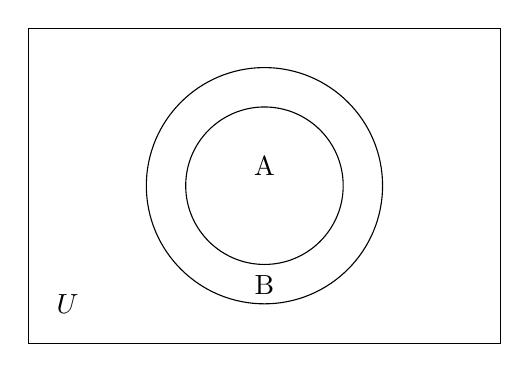
\begin{tikzpicture}
\draw (0,0) rectangle (6, 4);
\draw (3, 2) circle [radius=1.5];
\draw (3, 2) circle [radius=1];
\node at (0.5,0.5) {$U$};
\node [above] at (3,0.5) {B};
\node [below] at (3,2.5) {A};
\end{tikzpicture}
\end{center}

Note that for a set $A$ selected from a universe $U$:
\[A\subseteq U\]

Instead of using the quantifier definition for subset, we typically use an
implication form:
\[A\subseteq B\coloneqq a\in A\rightarrow a\in B\]
in other words, if $a$ is an element of $A$ then it must also be an element of
$B$.

By definition, a set is always a subset of itself: $A\subseteq A$. In fact, $A$
is referred to as the \emph{improper} subset of $A$. If we want $A$ to be a
subset of $B$ but not the same as $B$, then we write: $A\subset B$. In this
case, $A$ is called a \emph{proper} subset of B. Also by definition, the
empty set is a subset of any set: $\emptyset\subseteq A$. So, any set other
than the empty set always has at least two subsets: itself and the empty set.
The empty set only has one subset: itself.

\subsection*{Equality}

Two sets $A$ and $B$ are equal if they have the same elements; everything in
$A$ is in $B$ and everything in $B$ is in $A$. In other words, they are
subsets of each other:
\[A=B\coloneqq A\subseteq B\ and\ B\subseteq A\]
In terms of elements:
\[A=B\coloneqq a\in A\ \mbox{iff}\ a\in B\]
In other words, if an element $a$ is in $A$ then it must also be in $B$ (and
vice-versa), and if it is not in $A$ then it cannot be in $B$.

\subsection*{Operations}

Set operations are used to construct new sets from existing sets. We will be
concerned with three such operations:
\begin{itemize}
\item Union
\item Intersection
\item Difference
\end{itemize}
Although these operators are defined for two sets, they can be extended to
include more. In some cases in mathematics, the number of sets may even be
infinite (though not for our purposes).

\subsubsection*{Union}

The \emph{union} of two sets $A$ and $B$, denoted $A\cup B$, is the set
consisting of everything in $A$ or $B$; an element only needs to be in one
of the sets to be in the union:
\[A\cup B=\{x|x\in A\ \mbox{or}\ x\in B\}\]
The following Venn diagram demonstrates a union between two sets.

\begin{center}
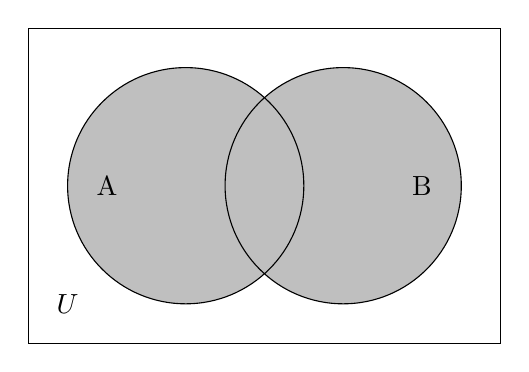
\begin{tikzpicture}
\def\setA{(2, 2) circle [radius=1.5]}
\def\setB{(4, 2) circle [radius=1.5]}
\draw (0,0) rectangle (6, 4);
\fill [lightgray] \setA;
\fill [lightgray] \setB;
\draw \setA;
\draw \setB;
\node at (0.5,0.5) {$U$};
\node at (1,2) {A};
\node at (5,2) {B};
\end{tikzpicture}
\end{center}

For example, let:
\begin{eqnarray*}
A &=& \{1, 2, 3\} \\
B &=& \{3, 4, 5\} \\
\end{eqnarray*}
The resulting union would be:
\[A\cup B=\{1, 2, 3, 4, 5\}\]
Note that even though the element `3' is in both A and B, it is only included
in the union once because set elements are distinct.

\subsubsection*{Intersection}

The \emph{intersection} of two sets $A$ and $B$, denoted $A\cap B$, is the set
consisting of everything that is in both $A$ and $B$; an element must be in both
to be in the intersection:
\[A\cap B=\{x|x\in A\ \mbox{and}\ x\in B\}\]
The following Venn diagram demonstrates an intersection between two sets.

\begin{center}
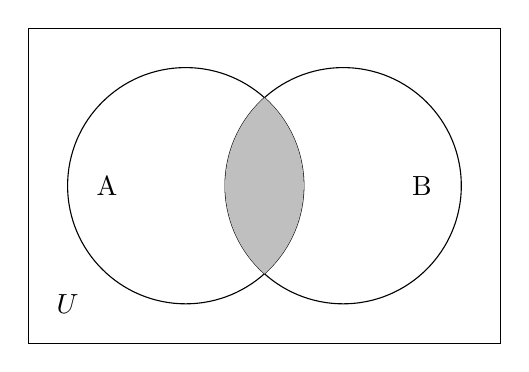
\begin{tikzpicture}
\def\setA{(2, 2) circle [radius=1.5]}
\def\setB{(4, 2) circle [radius=1.5]}
\draw (0,0) rectangle (6, 4);
\draw \setA;
\draw \setB;
\begin{scope}
\clip \setB;
\fill [lightgray] \setA;
\end{scope}
\node at (0.5,0.5) {$U$};
\node at (1,2) {A};
\node at (5,2) {B};
\end{tikzpicture}
\end{center}

Continuing with the previous example:
\[A\cap B=\{3\}\]
since the element `3' is the only element that is in both $A$ and $B$.

Sometimes, the intersection is the empty set; there are no elements in common.
For example, let:
\begin{eqnarray*}
A &=& \{1, 2, 3\} \\
B &=& \{4, 5, 6\} \\
\end{eqnarray*}
Now, $A\cap B=\emptyset$.

\subsubsection*{Difference}

You have probably encountered set unions and intersections before; however, set
difference may be new to you. The \emph{difference} between two sets $A$ and
$B$, denoted $A-B$, is the set consisting of everything that is in $A$ but not
in $B$; we start with the set $A$ and then remove any of its elements that are
also in $B$. Elements in $B$ that are not in $A$ are ignored:
\[A-B=\{x|x\in A\ \mbox{and}\ x\notin B\}\]
The following Venn diagram demonstrates the difference between $A$ and $B$:

\begin{center}
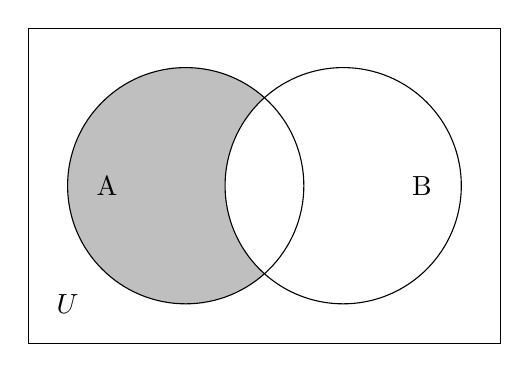
\begin{tikzpicture}
\def\setA{(2, 2) circle [radius=1.5]}
\def\setB{(4, 2) circle [radius=1.5]}
\draw (0,0) rectangle (6, 4);
\fill [lightgray] \setA;
\fill [white] \setB;
\draw \setA;
\draw \setB;
\node at (0.5,0.5) {$U$};
\node at (1,2) {A};
\node at (5,2) {B};
\end{tikzpicture}
\end{center}

For example, let:
\begin{eqnarray*}
A &=& \{1, 2, 3, 4, 5\} \\
B &=& \{3, 5, 6, 7\} \\
\end{eqnarray*}
\[A-B=\{1, 2, 4\}\]
We start with $A$ and then remove the elements `3' and `5' which are also in
$B$. We ignore the other elements in $B$ that are not in $A$ (`6' and `7').

Note the union and intersection operators are commutative, the difference
operator is not:
\begin{eqnarray*}
A\cup B &=& B\cup A \\
A\cap B &=& B\cap A \\
A-B &\ne& B-A \\
\end{eqnarray*}

\end{document}
